\chapter{REALM Demonstration}
% Main Gist 
% - Demonstrate OpenMC problem with REALM. 
% Structure 
% - realm demonstration of OpenMC Coupling for a toy problem. 
In this chapter, I demonstrate \gls{REALM}'s capabilities with a simple neutronics 
problem. 

\section{Problem Definition}
I explore how inhomogeneous fuel distributions impact $k_{eff}$ compared to 
homogenous fuel distributions that are customary in most reactor designs. 
The reactor core explored is a simple $20 \times 2 \times 2\ cm^3$ slab design
with reflective boundary conditions. 
The slab is divided into ten slices along the x axis resulting in 
$2 \times 2 \times 2\ cm^3$ slices. 
I use \gls{TRISO} fuel with a graphite moderator.
Each \gls{TRISO} particle has the same dimensions and material composition 
as in the \gls{FHR} benchmark (Figure \ref{fig:ahtr-triso}). 

The \gls{REALM} optimization problem's objective is to maximize $k_{eff}$, by 
varying the \gls{TRISO} particle packing fraction for each slice, while keeping 
total \gls{TRISO} particle packing fraction constant at 0.05. 
The \gls{TRISO} particle packing fraction's distribution across slices is 
governed by a sine equation: 
\begin{align}
    PF(x) &= a\ sin(bx + c) + 1 \\
    \intertext{where}
    a, b, c &= \mbox{constants that control sine function's shape} \nonumber \\
    x &= \mbox{midpoint value for each slice} \nonumber
\end{align}
The genetic algorithm varies the $a$, $b$ and $c$ variables. 
The packing fraction values are then normalized by the total packing fraction. 
Thus, for a packing fraction distribution of 
$PF(x) = 0.5\ sin(\frac{\pi}{3}x + \pi) + 1 $. 
The packing fraction for the ten slices are 0.0296, 0.0525, 0.0748, 0.0294, 
0.0530, 0.0746, 0.0292, 0.0534, 0.0744, 0.0290, respectively. 
Figure \ref{fig:triso_distribution} shows a plot of the sine curve, highlights 
the packing fraction at the respective midpoints, and an xz view of the slab
with varying packing fraction. 
\begin{figure}[]
    \centering
    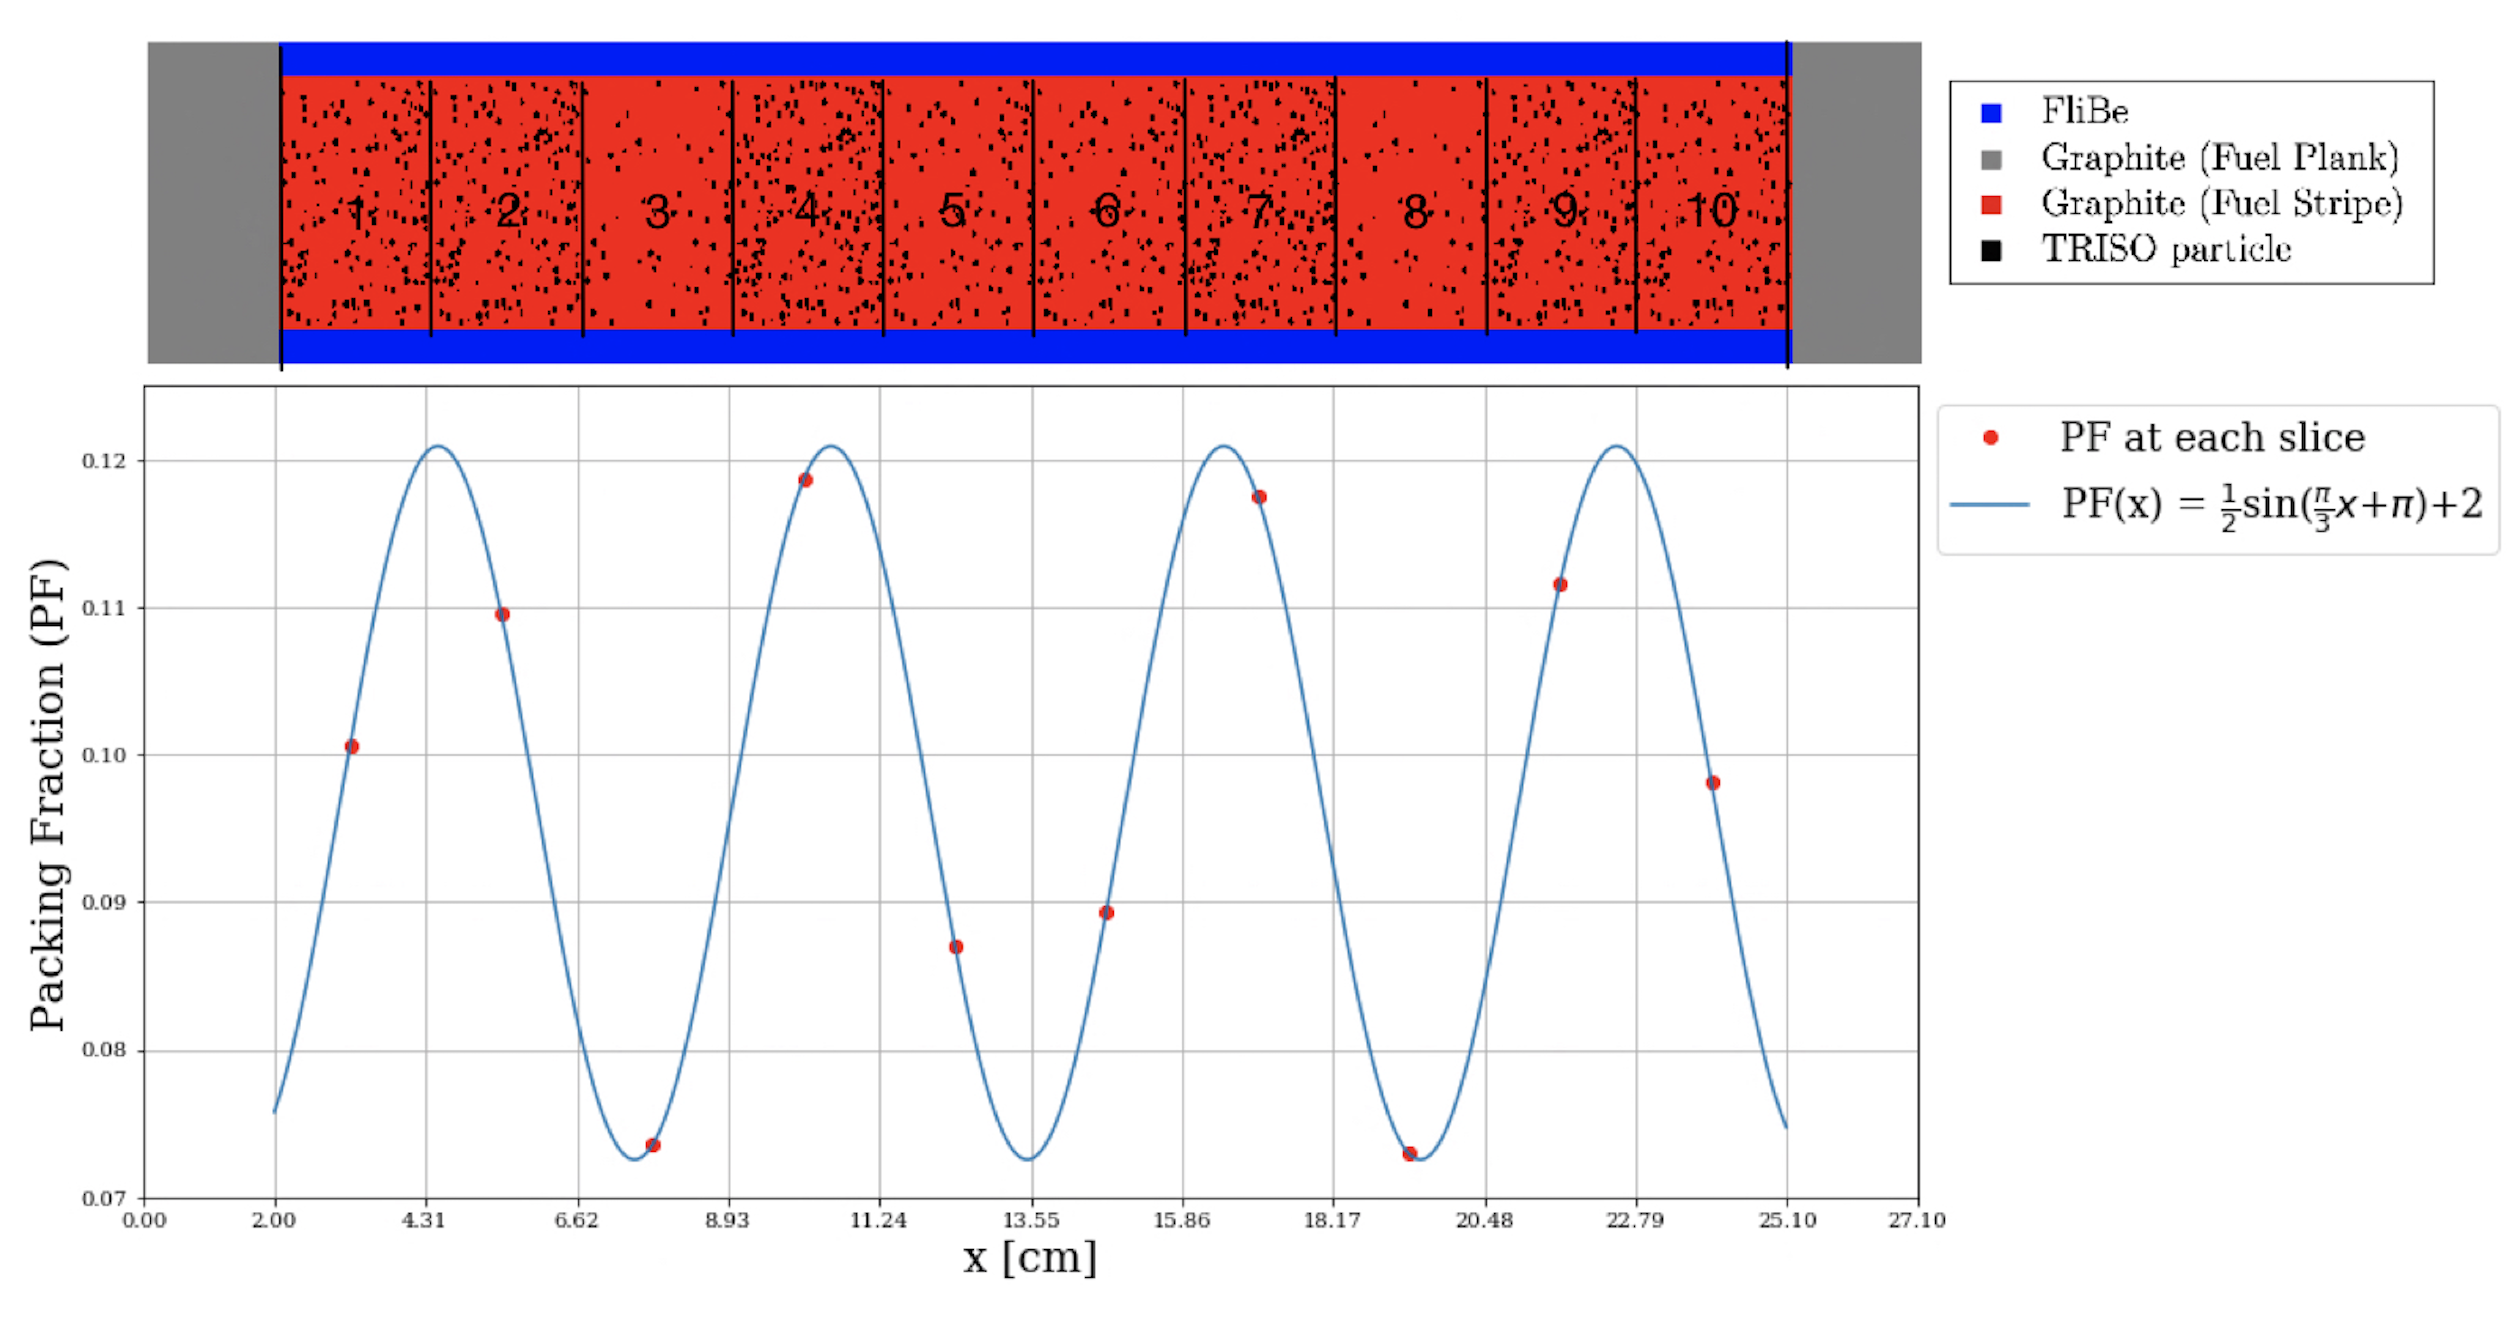
\includegraphics[width=\linewidth]{triso_distribution_sine.png} 
    \caption{TRISO}
    \label{fig:triso_distribution}
\end{figure}
The evaluator is OpenMC which is used to calculate $k_{eff}$. 


\section{Hyperparameter Search}
I conducted a coarse hyperparameter search with random sampling. 
I used random search over grid search because of the former's efficiency in 
high-dimensional spaces. 
Figure \ref{fig:random_vs_grid_sampling} illustrates how grid sampling gives 
even coverage in the original 2-d space, but provides inefficient coverage in 
projections onto either the x1 or x2 subspace.  
In contrast, random sampling has slightly less evenly distributed in the original 
space, but far more evenly distributed in the subspaces.
\begin{figure}[]
    \centering
    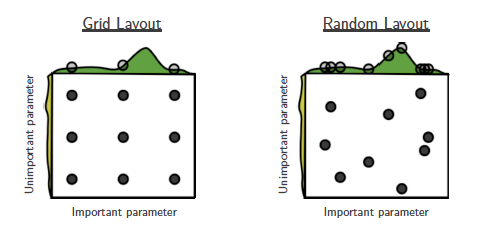
\includegraphics[width=0.8\linewidth]{random_vs_grid_sampling.png} 
    \caption{TRISO}
    \label{fig:random_vs_grid_sampling}
\end{figure}
The hyperparameters varied include: population size, number of generations, 
mutation probability, mating probability, selection operator, selection operator's 
k value, selection operator's tournament size, mutation operator, and mating 
operator.  

\section{Results}
